\chapter{Testing}

% \todo[inline]{
% Detailed descriptions of every test case are definitely not what is required here. What is important is to show that you adopted a sensible strategy that was, in principle, capable of testing the system adequately even if you did not have the time to test the system fully.

% Provide information in the body of your report and the appendix to explain the testing that has been performed. How does this testing address the requirements and design for the project?

% How comprehensive is the testing within the constraints of the project?  Are you testing the normal working behaviour? Are you testing the exceptional behaviour, e.g. error conditions? Are you testing security issues if they are relevant for your project? 

% Have you tested your system on ``real users''? For example, if your system is supposed to solve a problem for a business, then it would be appropriate to present your approach to involve the users in the testing process and to record the results that you obtained. Depending on the level of detail, it is likely that you would put any detailed results in an appendix.

% The following sections indicate some areas you might include. Other sections may be more appropriate to your project. 
% }

\section{Approach}
Testing is an extremely important element in developing any application. The approach used for this project used automated unit tests, static code analysis and \gls{linting} tests. For manual testing, acceptance tests on the completion of a feature were performed before merging into the main branch. Additionally, user tests of the whole system and memory inspection tests have been performed using the profiler Valgrind~\cite{valgrind}.

\section{Automated Testing}
A series of tests have been automated for the project. These tests are run on new commits pushed to the central repository. This is done using a webhook from Github to notify the automation platform Jenkins to run a new build. Jenkins\cite{jenkins} will then pull new changes from the repository for testing. 

The project is first tested by making sure it compiles without errors or any major warnings. The build time is recorded so that the developer can later see what changes had the largest impact and take appropriate action if required. Next the application unit tests are run with the results being output to XML files that are then read by Jenkins. These results are then formatted to show the number of passing and failing tests over time. Finally Cppcheck~\cite{Cppcheck} is run. This looks for common problems and mistakes in code such as unfreed memory or use of non-portable syntax and functions, such as syntax exclusive to GCC. Finally the results are fed back to be displayed on Github and as well as on a live dashboard (see figure~\ref{fig:ci_dashboard}). 

\begin{figure}
    \centering
    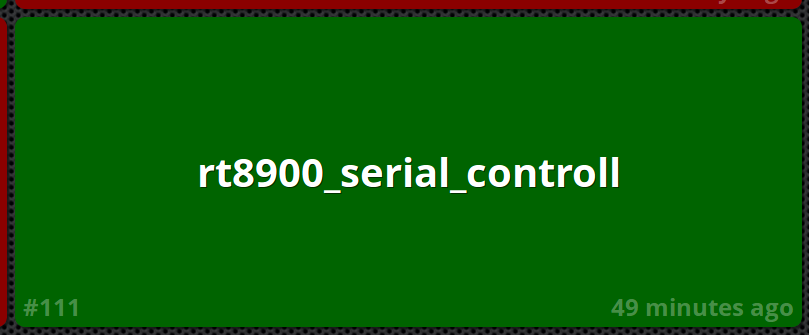
\includegraphics[width=0.5\textwidth]{img/CI_dashboard.png}
    \caption{A screenshot of the CI dashboard. This can be left open on a screen to track the build status. On failed builds this would turn red with a reason specified.}
    \label{fig:ci_dashboard}
\end{figure}

\begin{figure}
    \centering
    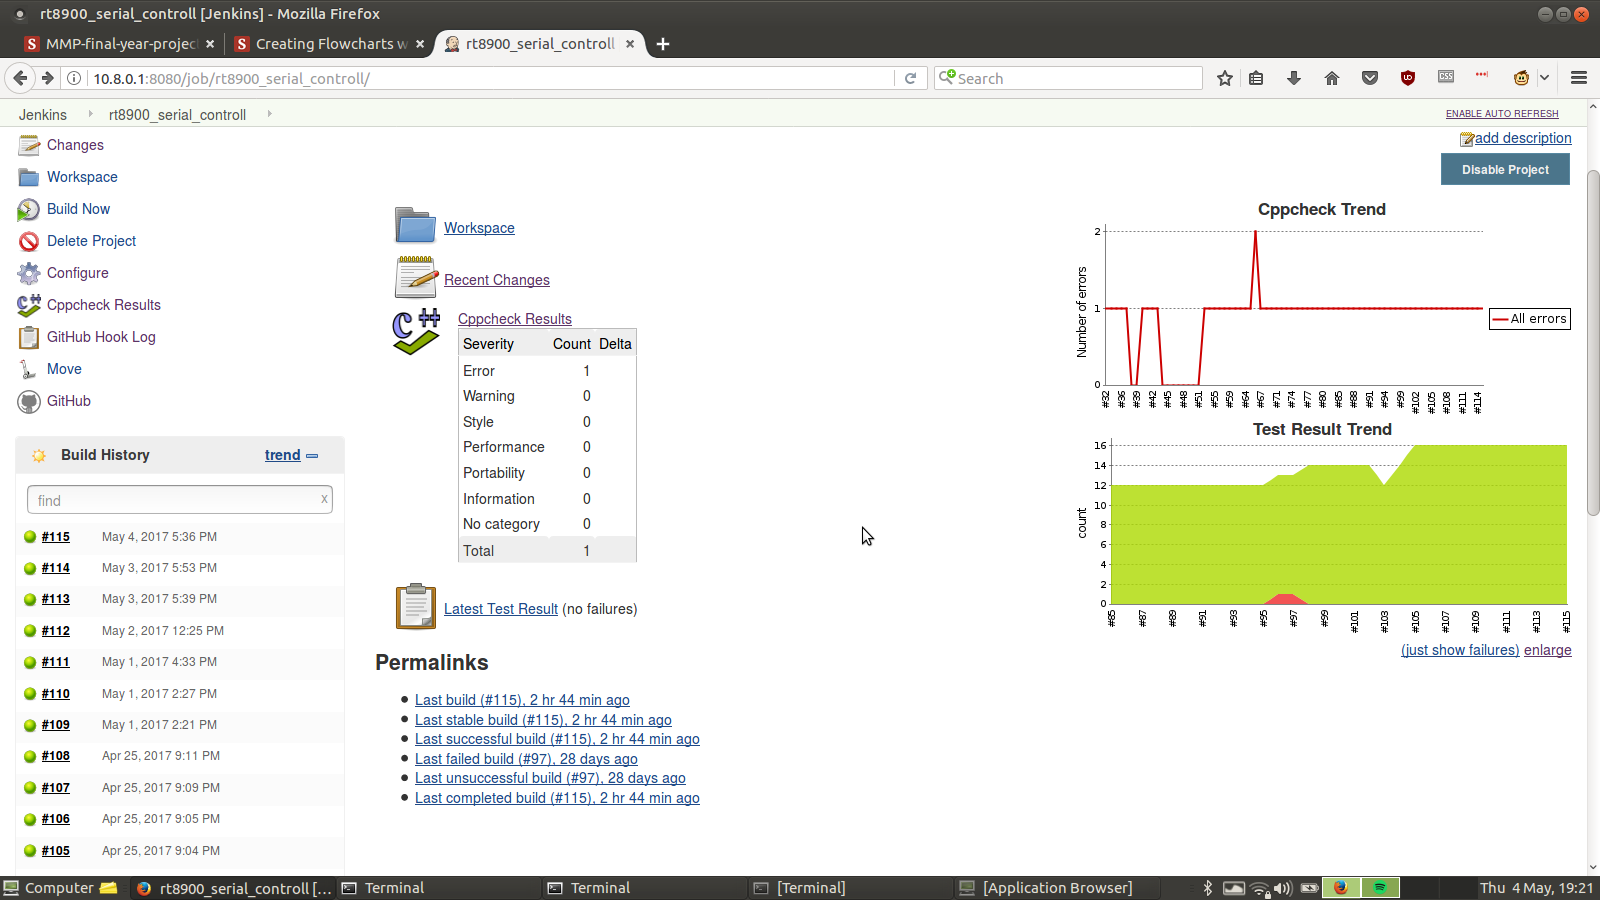
\includegraphics[width=1\textwidth]{img/jenkins_build.png}
    \caption[Jenkins build trends]{Jenkins showing test and error trends over time.}
    \label{fig:jenkins_build}
\end{figure}

\begin{figure}
    \centering
    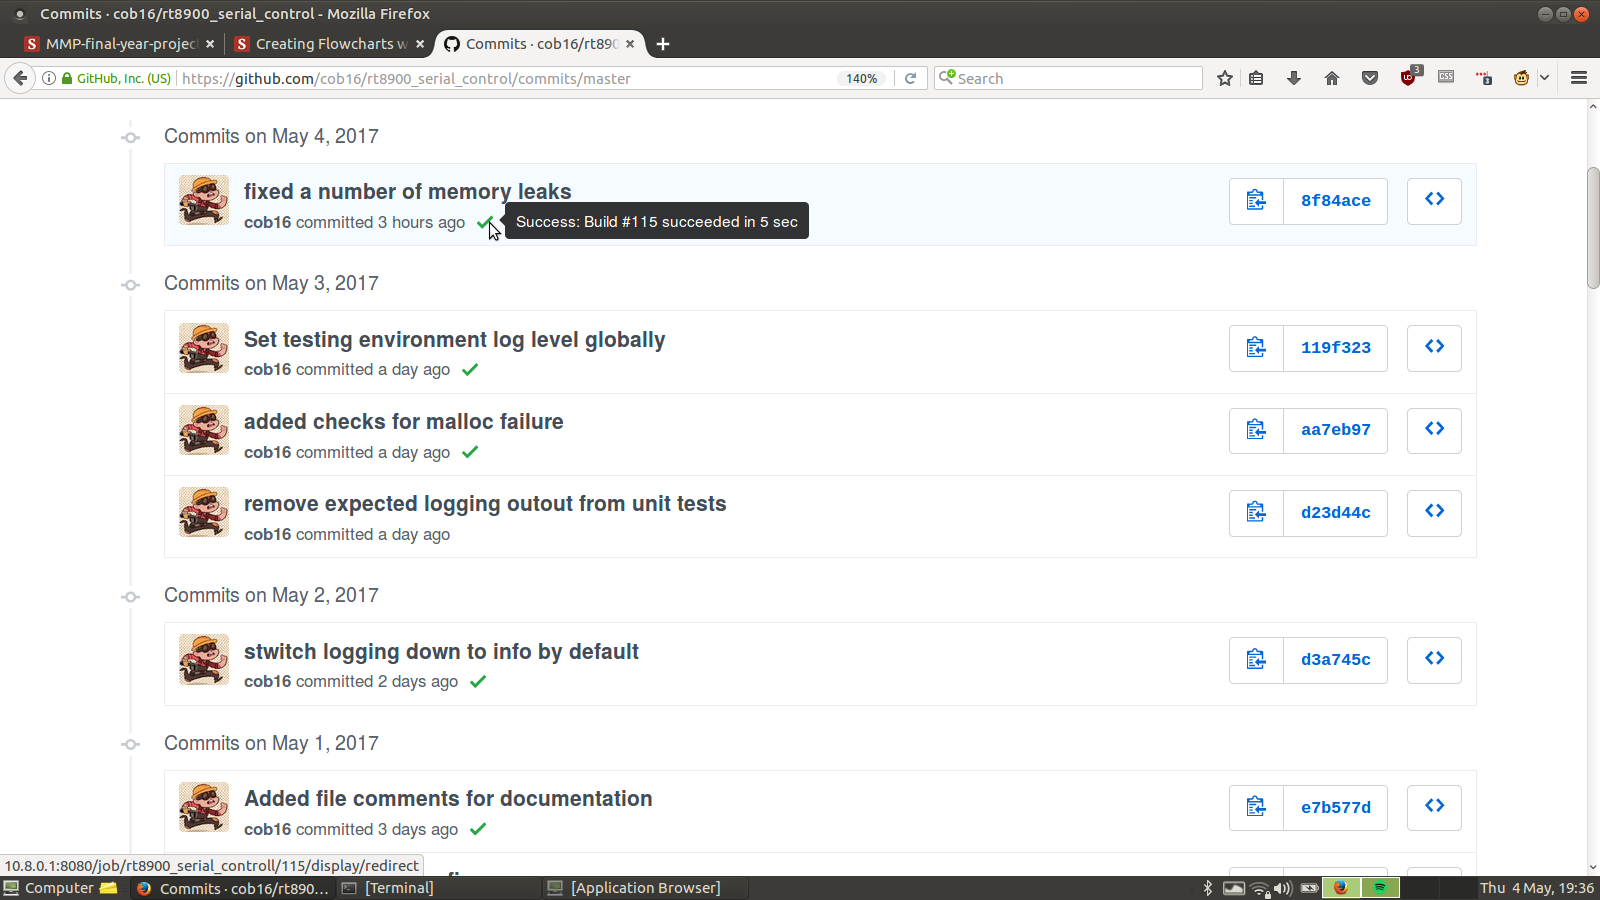
\includegraphics[width=1\textwidth]{img/github_commits.png}
    \caption[Tests on github]{Github commit list showing a tick on successful builds of each commit. This is useful historical information and is invaluable in preventing merges of unstable branches.}
    \label{fig:github_commits}
\end{figure}

\subsection{Unit Tests}
The project utilised unit tests throughout development (See appendix ~\ref{unit_test_output} for test output). This was an invaluable tool not only when re-factoring but allowed development of the application outside of the lab where the radio was held while still being able to test the program. Unit tests were primarily used to test the expected use-case as well as a number of important edge cases. For example if the pointer given was a null pointer the function should not de-reference it (otherwise the program would crash).

\section{Manual Testing}
Manual testing of the user shell was done by testing behaviour when expected and unexpected input was given. This was used to improve the user experience until a reasonably robust system had been made. User input is checked for the correct number of keywords and arguments. Arguments are safely cast to integers and range checked before being passed on to their corresponding functions. The input buffer will dynamically relocate to fit the input, up to a hard limit. The interrupt signal is handled from with in the application so that the program can be shutdown gracefully at any time.

\begin{figure}[]
    \centering
    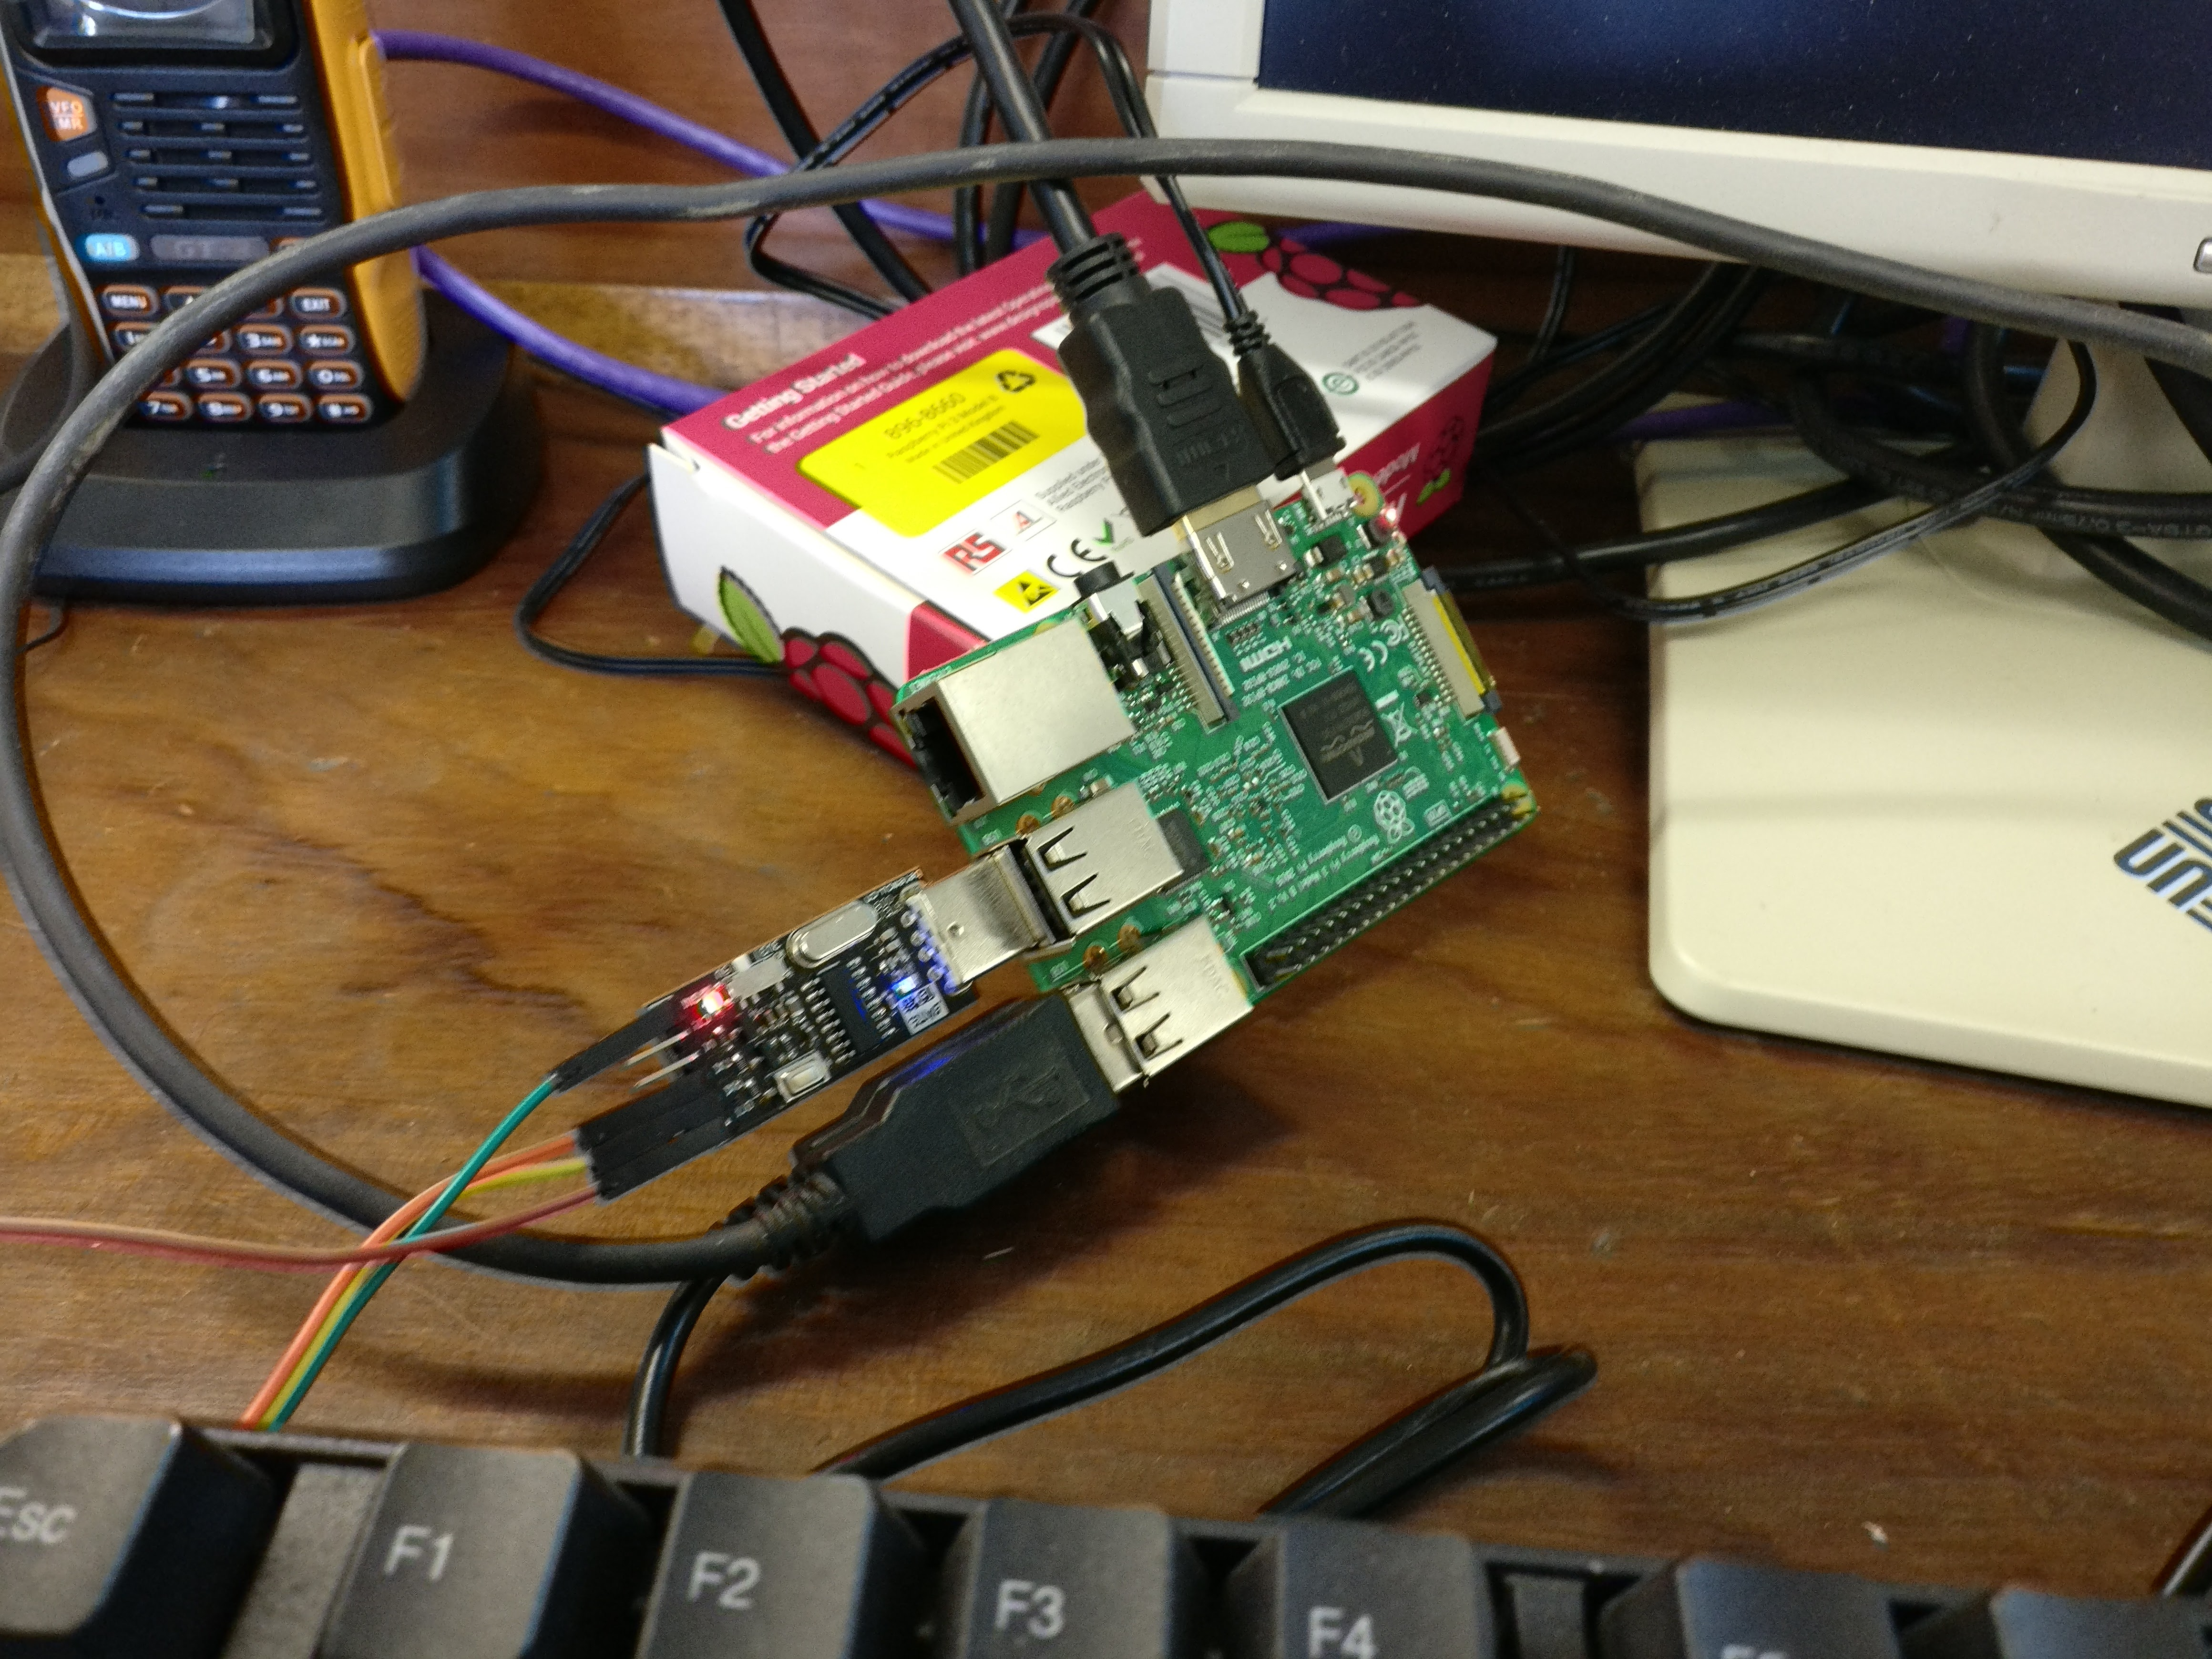
\includegraphics[width=1\textwidth]{img/raspberry_pi.jpg}
    \caption{A Raspberry Pi running the application}
    \label{fig:raspberry_pi}
\end{figure}

The application was also tested on a number of releases by watching a user with no prior experience with the system. Their feedback was accounted for by re-prioritising features as well as making tweaks to the interface to better meet users expectations. These tests were combined by compiling and running the program on a separate system (see figure~\ref{fig:raspberry_pi})to that used during development to ensure that all necessary files were included in Git.

Finally acceptance tests were conducted. Commands were checked to make sure their function worked as expected. This was done by cross-referencing the expected output with the output of the screen on the radio. The results of this are displayed in table~\ref{table:acceptance_tests}.

\begin{table}[]
\centering
\begin{tabular}{|p{0.1\textwidth}|p{0.8\textwidth}|l|}
\hline
Feature               & Acceptance test                                                                                                                          & Status     \\
\hline
\hline
Frequency             & As a user I can set any valid frequency I desire for both VFO's of the radio. I can also get the current set frequencies from the radio. & Complete   \\
\hline
Push to talk          & As a user I am able to transmit on frequencies that the radio permits. I am also able to check if the radio is transmitting.             & Complete   \\
\hline
Volume                & As a user I want to set the volumes of the radios independently.                                                                         & Complete   \\
\hline
Squelch               & As a user I want to customise the squelch levels of the radio to reduce the amount of background noise on my radio.                      & Complete   \\
\hline
Power                 & As a user I want to set the transmission power of each the radio.                                                                        & Complete   \\
\hline
Power on the radio & As a user I want the radio to automatically turn on when the application starts.                                                          & Incomplete \\
\hline
\end{tabular}
\caption[Acceptance testing]{Table of Acceptance tests and outcome}
\label{table:acceptance_tests}
\end{table}

\subsection{Memory profiling}
Valgrind\cite{valgrind} was used to check for memory leaks in the developed program using the following command.

\begin{minted}[breaklines]{bash}
valgrind --trace-children=yes --leak-check=full ./main/rt8900c -v5 /dev/ttyUSB0 
\end{minted}

This was an invaluable tool that found 4 leaks in the application. Its output also lists which function the memory was allocated to, making fixes easy. Massif was also used to measure the amount of memory that the application used (See figure~\ref{fig:memory_usage}). The peak memory usage of the application is 3.6 KiB. This peak occurs when a frequency is being dialled due to the large use of the sending queue to press each button in sequence. This is more than adequate for the current use-case, allowing for even the smallest microcontrollers to run the application.

\begin{minted}[breaklines]{bash}
valgrind --tool=massif ./rt8900_serial_control/cmake-build-debug/main/rt8900c -v5 /dev/ttyUSB0 
\end{minted}

\begin{figure}[H]
    \centering
    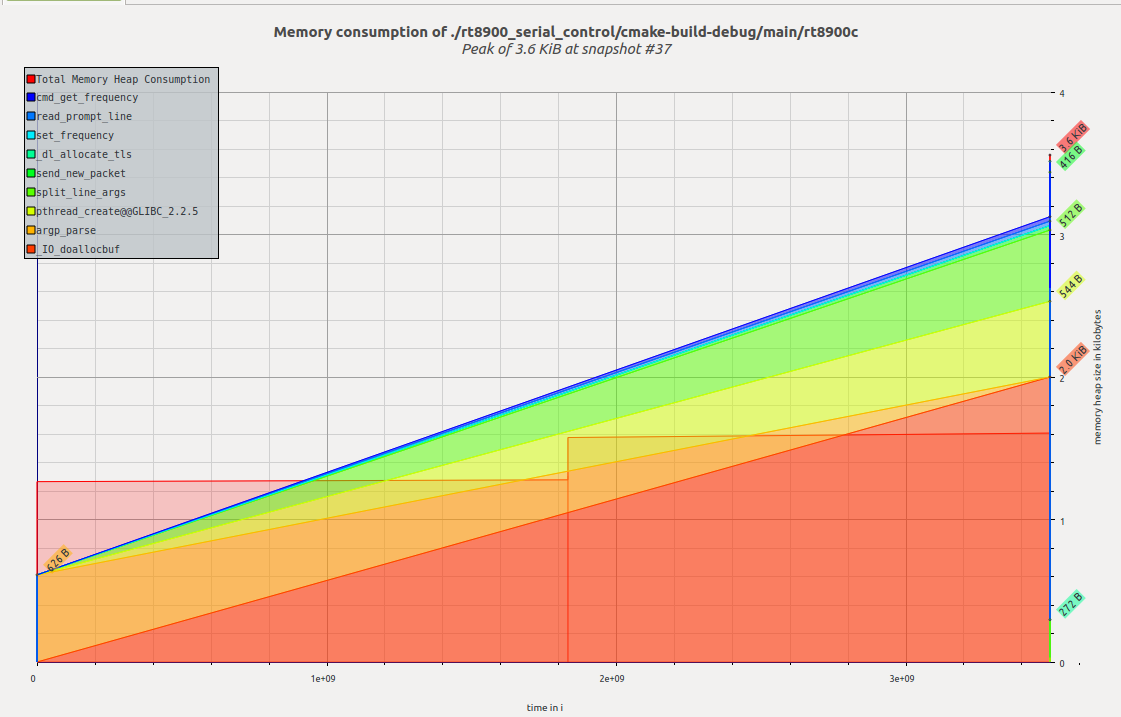
\includegraphics[width=1\textwidth]{img/memory_usage.png}
    \caption[Memory usage graph]{Memory usage of the application over time. This recording was done while the user tested every available function in the application.}
    \label{fig:memory_usage}
\end{figure}

\section{Known issues}
There were two known issues with the project at the time of submission. These issues were not deemed critical due to their current workarounds but are important improvements in development of the application.

\subsection*{Frequency validation}
Frequency validation follows the given list of frequencies from the user manual~\cite{user_manual}. However after testing, it was found that the right receiver supports only a subset of the frequencies that are listed. Further experimentation is required to discover this subset so that the validation can be correct for both receivers. This bug is limited in impact as upon receiving an invalid frequency the radio simply does nothing. In addition the user can see that the frequency was not changed from the output of the program.

\subsection*{Display packet reading}
\label{display_packet_reading}
Many functions that read and write packets currently have built in delays in order to give the radio time to send out a new display packet and to be processed by the reader thread. The true amount of time was not tested, therefore some functions sleep for as much as a second before continuing. This could be improved by implementing a getter function that blocks until a new packet is received. The problem with this is that this provides a risk if a new packet is never received (as the function would then block forever). Ideally the program should try to recover by timing out and falling back to a last known safe packet. More research and analysis of solutions into reading the display packet would have helped to mitigate this.

